\subsubsection*{(f) \textbf{(1,0 pontos)}}
\textit{Monte numa tabela comparativa a quantidade de operações (produtos e somas) realizadas.}

Baseando-se no resultado obtido a partir da execução dos algoritmos, foi construída a tabela \ref{tab:operacoes_comparativo}, que apresenta o número de operações necessárias para calcular as transformadas de Fourier discreta (DFT) e rápida (FFT) para diferentes tamanhos de amostra.

\begin{table}[ht]
    \centering
    \begin{tabular}{lccc}
    \textit{\textbf{Amostras}}            & \textbf{DFT (Ops)} & \textbf{FFT (Sums)} & \textbf{FFT (Mult)} \\
    \textit{32}                       & 1024                                & 160                  & 80                            \\
    \textit{32 + 32 0s}     & 4096                                & 384                  & 192                           \\
    \textit{64}                       & 4096                                & 384                  & 192                           \\
    \textit{64 + 64 0s}     & 16384                               & 896                  & 448                           \\
    \textit{128}                      & 16384                               & 896                  & 448                           \\
    \textit{128 + 128 0s}   & 65536                               & 2048                 & 1024                          \\
    \textit{256}                      & 65536                               & 2048                 & 1024                          \\
    \textit{256 + 256 0s}   & 262144                              & 4608                 & 2304                          \\
    \textit{512}                      & 262144                              & 4608                 & 2304                          \\
    \textit{512 + 512 0s}   & 1048576                             & 10240                & 5120                          \\
    \textit{1024}                     & 1048576                             & 10240                & 5120                          \\
    \textit{1024 + 1024 0s} & 4194304                             & 22528                & 11264                        
    \end{tabular}
    \caption{Comparativo da quantidade de operações (produtos e somas) realizadas em diferentes configurações de amostras.}
    \label{tab:operacoes_comparativo}
\end{table}


Baseando-se na Tabela \ref{tab:operacoes_comparativo}, foi realizo o plot dos seus valores na figura Figura \ref{fig:operations_comparison_graph}. Os resultados demonstram que a FFT é significativamente mais eficiente do que a DFT em termos de complexidade computacional, especialmente para grandes tamanhos de amostra.

\begin{figure}[H]
    \centering
    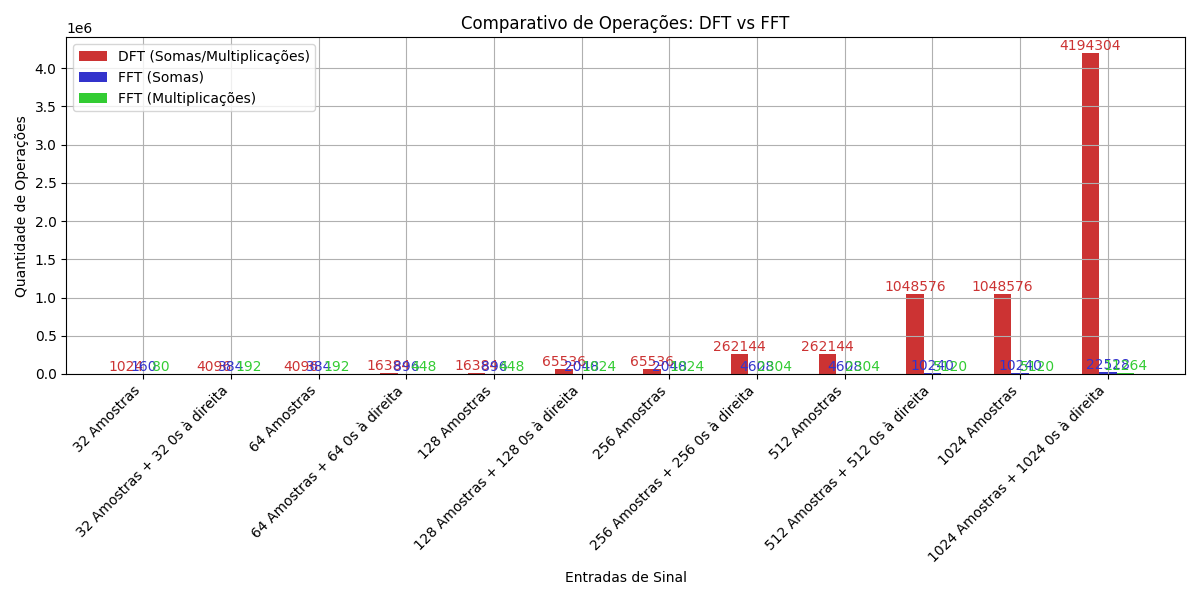
\includegraphics[width=1\linewidth]{03_experimental_analysis//assets/operations_comparison.png}
    \caption{Gráfico comparativo entre a quantidade de operações dos resultados}
    \label{fig:operations_comparison_graph}
\end{figure}

O comportamento do gráfico deixa claro as características do algoritmos, pois enquanto a DFT possui uma complexidade $O(N^2)$, a FFT possui a complexidade $O(N\log{N})$.

À medida que o número de amostras aumenta, a quantidade de operações cresce, mas a FFT realiza muito menos operações que a DFT, destacando sua maior eficiência. Apesar da diferença inicial, para as amostras pequenas (como 32), ser de cerca de 6.4x, essa diferença se torna cada vez mais significativa para amostras maiores.

Portanto, é possível observar que a FFT apresenta um crescimento mais suave nas operações de soma e multiplicação em comparação com a DFT.
